\subsection{Checks actually executed}
Analytical gradients were compared with central finite differences on all real and imaginary beamforming entries and all RIS phases for five random states. The step was $10^{-6}$ and the optimal receiver was recomputed at perturbed points. The maximum relative gradient error was $1.35e-10$. Independent generalized-eigenvalue receiver verification gave maximum relative error $1.17e-15$. A separate 128-instance zero-phase initialization test accepted 103 cases; failures were retained. The accepted power limit and phase modulus were satisfied to floating-point tolerance.

\subsection{Held-out simulation results}
Table~\ref{tab:results} uses 128 held-out geometries. Learned-method entries average the three training seeds; conditional SCNR averages use each model's own feasible subset and must not be interpreted as paired comparisons. ``Feasible'' refers to nominal communication QoS and hardware constraints, not a sensing detection guarantee. No algorithm repairs failed initializations in this prototype.

\begin{table}[!htbp]\centering\small
\begin{tabular}{lrrrr}\toprule
Method & Feasible (\%) & Mean SCNR (dB) & Median (ms) & p95 (ms)\\\midrule
Initialization & 81.25 & -5.21 & 0.31 & 0.53 \\
Fixed steps (8) & 81.25 & 2.36 & 3.74 & 5.89 \\
Learn before & 82.29 & 2.15 & 3.85 & 6.20 \\
Learn inside & 81.25 & 2.84 & 3.76 & 5.99 \\
Before + inside & 81.77 & 2.66 & 3.84 & 6.54 \\
Backtracking (80) & 81.25 & 3.16 & 126.62 & 179.13 \\
\bottomrule\end{tabular}
\caption{Actual synthetic test results and batch-one solver timings. Learned timing entries are means of per-seed medians/p95 values, not pooled quantiles.}\label{tab:results}\end{table}

Runtime is measured with \texttt{perf\_counter} on this shared Linux CPU environment using NumPy complex128 and one OpenBLAS thread. Each method uses three repetitions over 32 batch-one inputs. Timing includes initialization, receiver solves, gradient steps, power repair, candidate evaluation, and final checks. It excludes offline learning and synthetic channel/feature construction. It also excludes sensing acquisition, channel estimation, RIS configuration, and queueing, none of which is simulated. Consequently these numbers are solver timings, not end-to-end deployment latency. Median synthetic input preparation took 0.119 ms; this is not an estimator timing. Offline training of all nine learned models took 61.21 s.

On geometries feasible for both the learned and fixed-step methods, the seed-averaged paired SCNR gain was 0.479 dB for inside-only learning, 0.322 dB for combined before/inside learning, and -0.104 dB for before-only learning. The corresponding geometry-bootstrap 95\% intervals were [0.370, 0.600], [0.213, 0.436], and [-0.221, 0.006] dB. These intervals hold the three trained models fixed and do not capture all training-distribution or model uncertainty.

The combined architecture did not consistently exceed inside-only learning. Before-only learning traded a small feasibility change for lower paired sensing quality. There is no demonstrated runtime reduction relative to the equally shallow eight-step baseline; the 80-step reference spends more time and attains higher average sensing quality. The results support a modest learned-step benefit in this pilot, not a general L2O superiority claim.

\begin{figure}[!htbp]\centering
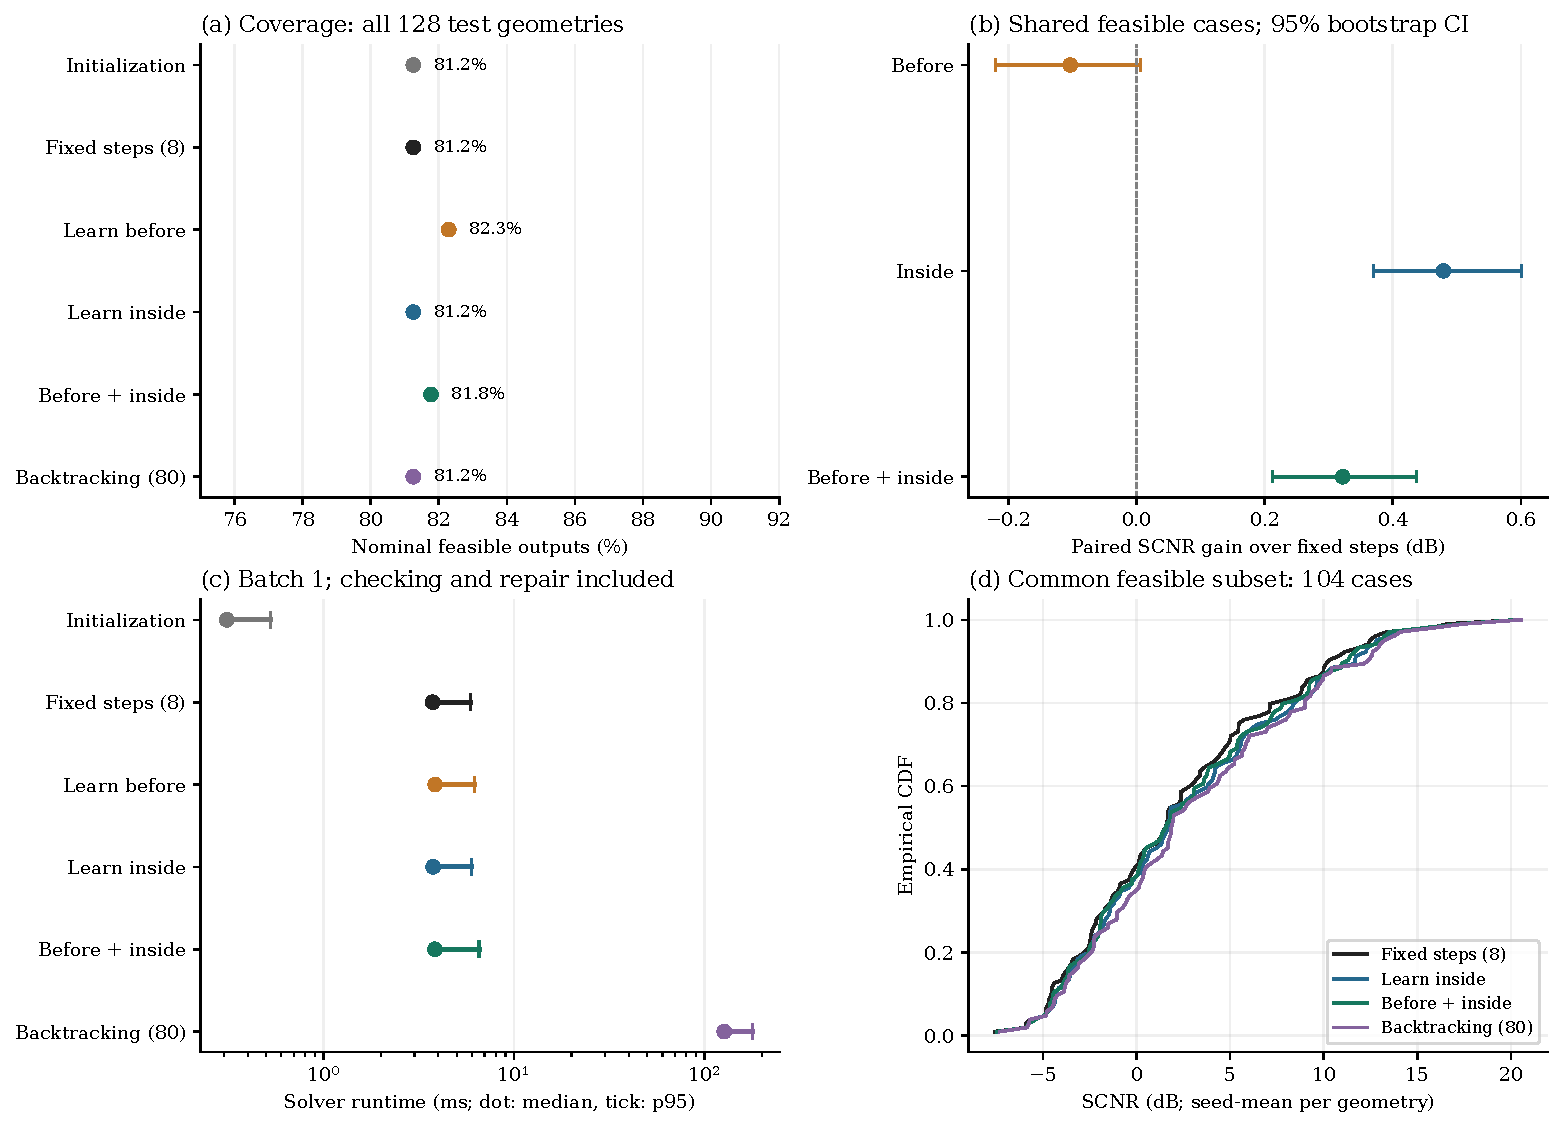
\includegraphics[width=\linewidth]{results/simulation-summary.pdf}
\caption{Measured results from this prototype. Coverage retains failed cases; paired gains and the CDF use shared-feasible subsets. Confidence intervals resample geometries with trained models held fixed.}\end{figure}

\subsection{Clutter shift and dimension diagnostic}
The shifted test multiplies clutter RCS by three and concentrates clutter around the target; it also uses new user and target geometries. It is therefore not a paired intervention on the same scenes. Inside-only learning retained an average paired improvement of 0.465 dB over fixed steps on their shared feasible cases; combined learning gave 0.323 dB. Neither result establishes robust feasibility under unknown channel or clutter errors.
An additional frozen-seed-17 diagnostic changes $(N,M)$ from $(6,12)$ to $(12,24)$ and $(24,48)$, retaining $K=2$ and fixed physical apertures. It uses 32 fresh instances at each size, with no retraining. It tests execution and limited dimension transfer only; it does not validate arbitrary-user scalability or array hardware physics.
\begin{center}\small\begin{tabular}{rrlrr}\toprule
$N$ & $M$ & Method & Feasible / 32 & Median (ms)\\\midrule
6 & 12 & fixed8 & 26 & 3.70 \\
6 & 12 & combined17 & 26 & 3.66 \\
12 & 24 & fixed8 & 32 & 4.07 \\
12 & 24 & combined17 & 32 & 4.09 \\
24 & 48 & fixed8 & 32 & 6.15 \\
24 & 48 & combined17 & 32 & 5.98 \\
\bottomrule\end{tabular}\end{center}
An independent covariance check with 100,000 random symbol/scatterer draws produced SCNR relative error 0.0051 against the analytical expression. This checks the assumed ensemble covariance model, not its validity for measured clutter.
\begin{figure}[!htbp]\centering
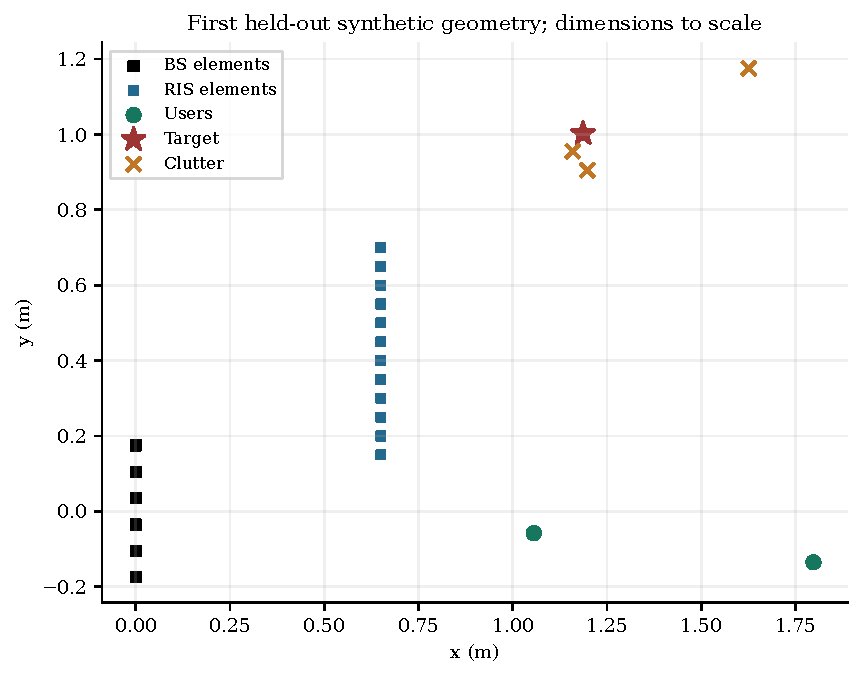
\includegraphics[width=.75\linewidth]{results/simulated-geometry.pdf}
\caption{Coordinates of the first held-out case used by the simulator. This figure is generated from the saved test dataset, not an illustrative performance claim.}\end{figure}
